% Options for packages loaded elsewhere
\PassOptionsToPackage{unicode}{hyperref}
\PassOptionsToPackage{hyphens}{url}
%
\documentclass[
]{article}
\usepackage{amsmath,amssymb}
\usepackage{iftex}
\ifPDFTeX
  \usepackage[T1]{fontenc}
  \usepackage[utf8]{inputenc}
  \usepackage{textcomp} % provide euro and other symbols
\else % if luatex or xetex
  \usepackage{unicode-math} % this also loads fontspec
  \defaultfontfeatures{Scale=MatchLowercase}
  \defaultfontfeatures[\rmfamily]{Ligatures=TeX,Scale=1}
\fi
\usepackage{lmodern}
\ifPDFTeX\else
  % xetex/luatex font selection
\fi
% Use upquote if available, for straight quotes in verbatim environments
\IfFileExists{upquote.sty}{\usepackage{upquote}}{}
\IfFileExists{microtype.sty}{% use microtype if available
  \usepackage[]{microtype}
  \UseMicrotypeSet[protrusion]{basicmath} % disable protrusion for tt fonts
}{}
\makeatletter
\@ifundefined{KOMAClassName}{% if non-KOMA class
  \IfFileExists{parskip.sty}{%
    \usepackage{parskip}
  }{% else
    \setlength{\parindent}{0pt}
    \setlength{\parskip}{6pt plus 2pt minus 1pt}}
}{% if KOMA class
  \KOMAoptions{parskip=half}}
\makeatother
\usepackage{xcolor}
\usepackage[margin=1in]{geometry}
\usepackage{color}
\usepackage{fancyvrb}
\newcommand{\VerbBar}{|}
\newcommand{\VERB}{\Verb[commandchars=\\\{\}]}
\DefineVerbatimEnvironment{Highlighting}{Verbatim}{commandchars=\\\{\}}
% Add ',fontsize=\small' for more characters per line
\usepackage{framed}
\definecolor{shadecolor}{RGB}{248,248,248}
\newenvironment{Shaded}{\begin{snugshade}}{\end{snugshade}}
\newcommand{\AlertTok}[1]{\textcolor[rgb]{0.94,0.16,0.16}{#1}}
\newcommand{\AnnotationTok}[1]{\textcolor[rgb]{0.56,0.35,0.01}{\textbf{\textit{#1}}}}
\newcommand{\AttributeTok}[1]{\textcolor[rgb]{0.13,0.29,0.53}{#1}}
\newcommand{\BaseNTok}[1]{\textcolor[rgb]{0.00,0.00,0.81}{#1}}
\newcommand{\BuiltInTok}[1]{#1}
\newcommand{\CharTok}[1]{\textcolor[rgb]{0.31,0.60,0.02}{#1}}
\newcommand{\CommentTok}[1]{\textcolor[rgb]{0.56,0.35,0.01}{\textit{#1}}}
\newcommand{\CommentVarTok}[1]{\textcolor[rgb]{0.56,0.35,0.01}{\textbf{\textit{#1}}}}
\newcommand{\ConstantTok}[1]{\textcolor[rgb]{0.56,0.35,0.01}{#1}}
\newcommand{\ControlFlowTok}[1]{\textcolor[rgb]{0.13,0.29,0.53}{\textbf{#1}}}
\newcommand{\DataTypeTok}[1]{\textcolor[rgb]{0.13,0.29,0.53}{#1}}
\newcommand{\DecValTok}[1]{\textcolor[rgb]{0.00,0.00,0.81}{#1}}
\newcommand{\DocumentationTok}[1]{\textcolor[rgb]{0.56,0.35,0.01}{\textbf{\textit{#1}}}}
\newcommand{\ErrorTok}[1]{\textcolor[rgb]{0.64,0.00,0.00}{\textbf{#1}}}
\newcommand{\ExtensionTok}[1]{#1}
\newcommand{\FloatTok}[1]{\textcolor[rgb]{0.00,0.00,0.81}{#1}}
\newcommand{\FunctionTok}[1]{\textcolor[rgb]{0.13,0.29,0.53}{\textbf{#1}}}
\newcommand{\ImportTok}[1]{#1}
\newcommand{\InformationTok}[1]{\textcolor[rgb]{0.56,0.35,0.01}{\textbf{\textit{#1}}}}
\newcommand{\KeywordTok}[1]{\textcolor[rgb]{0.13,0.29,0.53}{\textbf{#1}}}
\newcommand{\NormalTok}[1]{#1}
\newcommand{\OperatorTok}[1]{\textcolor[rgb]{0.81,0.36,0.00}{\textbf{#1}}}
\newcommand{\OtherTok}[1]{\textcolor[rgb]{0.56,0.35,0.01}{#1}}
\newcommand{\PreprocessorTok}[1]{\textcolor[rgb]{0.56,0.35,0.01}{\textit{#1}}}
\newcommand{\RegionMarkerTok}[1]{#1}
\newcommand{\SpecialCharTok}[1]{\textcolor[rgb]{0.81,0.36,0.00}{\textbf{#1}}}
\newcommand{\SpecialStringTok}[1]{\textcolor[rgb]{0.31,0.60,0.02}{#1}}
\newcommand{\StringTok}[1]{\textcolor[rgb]{0.31,0.60,0.02}{#1}}
\newcommand{\VariableTok}[1]{\textcolor[rgb]{0.00,0.00,0.00}{#1}}
\newcommand{\VerbatimStringTok}[1]{\textcolor[rgb]{0.31,0.60,0.02}{#1}}
\newcommand{\WarningTok}[1]{\textcolor[rgb]{0.56,0.35,0.01}{\textbf{\textit{#1}}}}
\usepackage{graphicx}
\makeatletter
\def\maxwidth{\ifdim\Gin@nat@width>\linewidth\linewidth\else\Gin@nat@width\fi}
\def\maxheight{\ifdim\Gin@nat@height>\textheight\textheight\else\Gin@nat@height\fi}
\makeatother
% Scale images if necessary, so that they will not overflow the page
% margins by default, and it is still possible to overwrite the defaults
% using explicit options in \includegraphics[width, height, ...]{}
\setkeys{Gin}{width=\maxwidth,height=\maxheight,keepaspectratio}
% Set default figure placement to htbp
\makeatletter
\def\fps@figure{htbp}
\makeatother
\setlength{\emergencystretch}{3em} % prevent overfull lines
\providecommand{\tightlist}{%
  \setlength{\itemsep}{0pt}\setlength{\parskip}{0pt}}
\setcounter{secnumdepth}{-\maxdimen} % remove section numbering
\ifLuaTeX
  \usepackage{selnolig}  % disable illegal ligatures
\fi
\IfFileExists{bookmark.sty}{\usepackage{bookmark}}{\usepackage{hyperref}}
\IfFileExists{xurl.sty}{\usepackage{xurl}}{} % add URL line breaks if available
\urlstyle{same}
\hypersetup{
  pdftitle={Projeto Final},
  hidelinks,
  pdfcreator={LaTeX via pandoc}}

\title{Projeto Final}
\author{Nome: Sofia Ferreira\\
E-mail:
\href{mailto:sofia.f@aluno.ufabc.edu.br}{\nolinkurl{sofia.f@aluno.ufabc.edu.br}}

Nome: Pedro Henrique Donassan de Macedo\\
E-mail:
\href{mailto:pedro.donassan@aluno.ufabc.edu.br}{\nolinkurl{pedro.donassan@aluno.ufabc.edu.br}}

Nome:\\
E-mail:

Nome:\\
E-mail:

Nome:\\
E-mail:

Nome:\\
E-mail:\\
(Não é preciso informar os RAs)}
\date{14 agosto, 2023}

\begin{document}
\maketitle

\hypertarget{section}{%
\section{}\label{section}}

\begin{Shaded}
\begin{Highlighting}[]
\DocumentationTok{\#\# Introdução}
\end{Highlighting}
\end{Shaded}

\begin{Shaded}
\begin{Highlighting}[]
\FunctionTok{library}\NormalTok{(tidyverse)}
\FunctionTok{library}\NormalTok{(tidymodels)}
\FunctionTok{library}\NormalTok{(mlbench)}
\FunctionTok{library}\NormalTok{(GGally)}
\FunctionTok{library}\NormalTok{(corrplot)}
\FunctionTok{library}\NormalTok{(vip)}
\FunctionTok{library}\NormalTok{(janitor)}

\FunctionTok{library}\NormalTok{(rpart.plot)}
\FunctionTok{library}\NormalTok{(randomForest)}
\end{Highlighting}
\end{Shaded}

\begin{Shaded}
\begin{Highlighting}[]
\NormalTok{data }\OtherTok{\textless{}{-}} \FunctionTok{read.csv}\NormalTok{(}
    \StringTok{"Sleep\_health\_and\_lifestyle\_dataset.csv"}\NormalTok{, }
    \AttributeTok{header=}\ConstantTok{TRUE}\NormalTok{, }
    \AttributeTok{sep =} \StringTok{","}\NormalTok{, }
    \AttributeTok{row.names =} \ConstantTok{NULL}\NormalTok{, }
    \AttributeTok{quote =} \StringTok{"}\SpecialCharTok{\textbackslash{}"}\StringTok{"}\NormalTok{) }

\NormalTok{data }\OtherTok{\textless{}{-}}\NormalTok{ data }\SpecialCharTok{\%\textgreater{}\%} \FunctionTok{clean\_names}\NormalTok{() }\CommentTok{\#Formatando nome das colunas}

\NormalTok{data }\OtherTok{\textless{}{-}} \FunctionTok{separate}\NormalTok{(data, blood\_pressure, }\AttributeTok{into =} \FunctionTok{c}\NormalTok{(}\StringTok{"systolic\_pressure"}\NormalTok{, }\StringTok{"diastolic\_pressure"}\NormalTok{), }\AttributeTok{sep =} \StringTok{"/"}\NormalTok{) }\CommentTok{\#Transformando pressão sanguínea em 2 variáveis numericas}
\NormalTok{data}\SpecialCharTok{$}\NormalTok{systolic\_pressure }\OtherTok{\textless{}{-}} \FunctionTok{as.numeric}\NormalTok{(data}\SpecialCharTok{$}\NormalTok{systolic\_pressure)}
\NormalTok{data}\SpecialCharTok{$}\NormalTok{diastolic\_pressure }\OtherTok{\textless{}{-}} \FunctionTok{as.numeric}\NormalTok{(data}\SpecialCharTok{$}\NormalTok{diastolic\_pressure)}

\NormalTok{data}\SpecialCharTok{$}\NormalTok{gender }\OtherTok{\textless{}{-}} \FunctionTok{as.factor}\NormalTok{(data}\SpecialCharTok{$}\NormalTok{gender)}
\NormalTok{data}\SpecialCharTok{$}\NormalTok{occupation }\OtherTok{\textless{}{-}} \FunctionTok{as.factor}\NormalTok{(data}\SpecialCharTok{$}\NormalTok{occupation)}
\NormalTok{data}\SpecialCharTok{$}\NormalTok{bmi\_category }\OtherTok{\textless{}{-}} \FunctionTok{as.factor}\NormalTok{(data}\SpecialCharTok{$}\NormalTok{bmi\_category)}
\CommentTok{\#data$blood\_pressure \textless{}{-} as.factor(data$blood\_pressure)}
\NormalTok{data}\SpecialCharTok{$}\NormalTok{sleep\_disorder }\OtherTok{\textless{}{-}} \FunctionTok{as.factor}\NormalTok{(data}\SpecialCharTok{$}\NormalTok{sleep\_disorder)}

\NormalTok{SleepData }\OtherTok{\textless{}{-}} \FunctionTok{as\_tibble}\NormalTok{(data) }
\FunctionTok{ggpairs}\NormalTok{(SleepData, }\AttributeTok{columns =} \FunctionTok{c}\NormalTok{(}\StringTok{"age"}\NormalTok{, }\StringTok{"sleep\_duration"}\NormalTok{, }\StringTok{"quality\_of\_sleep"}\NormalTok{, }\StringTok{"physical\_activity\_level"}\NormalTok{, }\StringTok{"stress\_level"}\NormalTok{, }\StringTok{"heart\_rate"}\NormalTok{, }\StringTok{"daily\_steps"}\NormalTok{, }\StringTok{"systolic\_pressure"}\NormalTok{, }\StringTok{"diastolic\_pressure"}\NormalTok{))}
\end{Highlighting}
\end{Shaded}

\begin{center}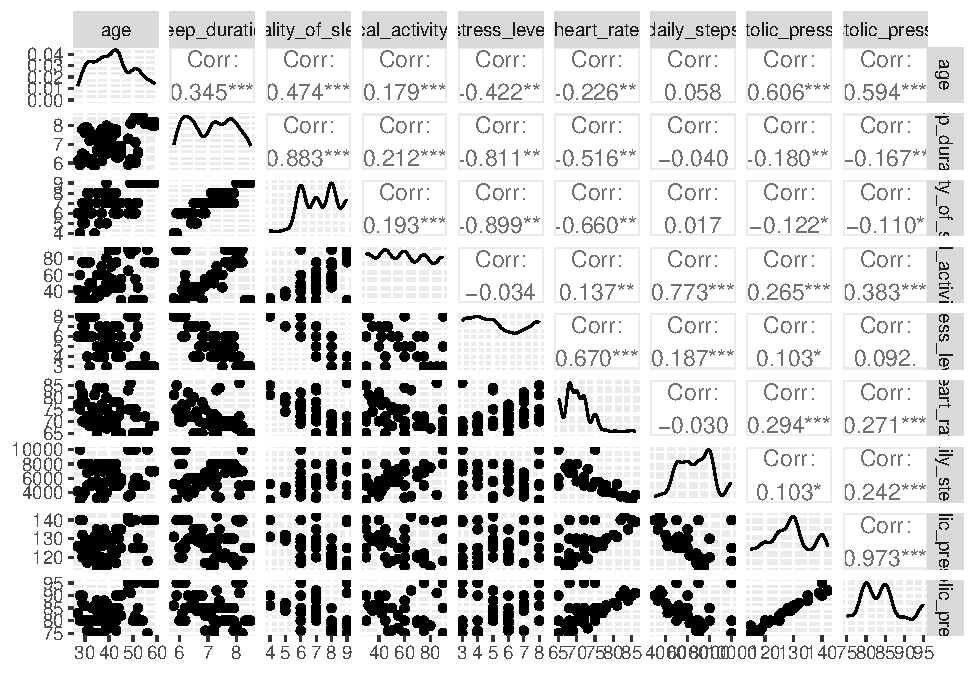
\includegraphics[width=0.6\linewidth]{projeto_files/figure-latex/pt. 2 -1} \end{center}

\begin{Shaded}
\begin{Highlighting}[]
\NormalTok{data }\SpecialCharTok{\%\textgreater{}\%} \FunctionTok{na.omit}\NormalTok{() }\SpecialCharTok{\%\textgreater{}\%} \FunctionTok{select\_if}\NormalTok{(is.numeric) }\SpecialCharTok{\%\textgreater{}\%} \FunctionTok{cor}\NormalTok{() }\SpecialCharTok{\%\textgreater{}\%}\NormalTok{ corrplot}\SpecialCharTok{::}\FunctionTok{corrplot}\NormalTok{(}\AttributeTok{tl.cex =} \FloatTok{0.5}\NormalTok{) }\CommentTok{\#Printando matriz de correlação}
\end{Highlighting}
\end{Shaded}

\begin{center}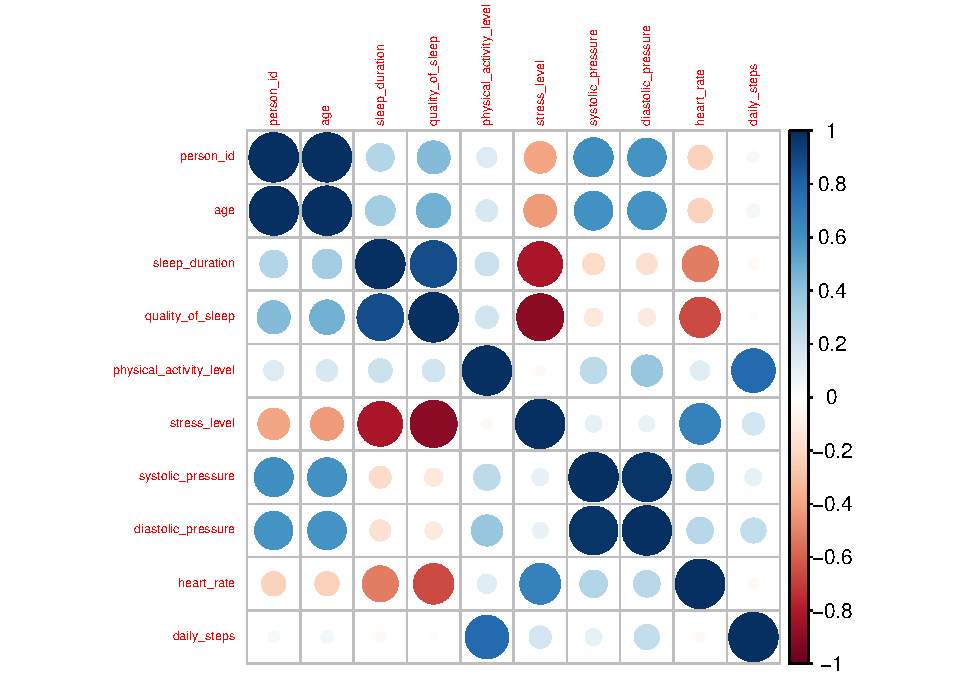
\includegraphics[width=0.6\linewidth]{projeto_files/figure-latex/pt. 2 -2} \end{center}

\begin{Shaded}
\begin{Highlighting}[]
\CommentTok{\#Split para todos os modelos}
\FunctionTok{set.seed}\NormalTok{(}\DecValTok{123}\NormalTok{) }\CommentTok{\# para reprodutibilidade}
\NormalTok{data\_split }\OtherTok{\textless{}{-}} \FunctionTok{initial\_split}\NormalTok{(SleepData, }\AttributeTok{prop =} \FloatTok{0.8}\NormalTok{)}
\NormalTok{train\_data }\OtherTok{\textless{}{-}} \FunctionTok{training}\NormalTok{(data\_split)}
\NormalTok{test\_data }\OtherTok{\textless{}{-}} \FunctionTok{testing}\NormalTok{(data\_split)}

\CommentTok{\#Cv para todos os modelos}
\FunctionTok{set.seed}\NormalTok{(}\DecValTok{123}\NormalTok{) }\CommentTok{\# para reprodutibilidade}
\NormalTok{cv\_folds }\OtherTok{\textless{}{-}} \FunctionTok{vfold\_cv}\NormalTok{(train\_data, }\AttributeTok{v =} \DecValTok{5}\NormalTok{) }\CommentTok{\# 5 Folds pois o dataset é pequeno}

\CommentTok{\#Recipe para todos os modelos}
\NormalTok{rec }\OtherTok{\textless{}{-}} \FunctionTok{recipe}\NormalTok{(sleep\_disorder }\SpecialCharTok{\textasciitilde{}}\NormalTok{ ., }\AttributeTok{data =}\NormalTok{ train\_data) }\SpecialCharTok{\%\textgreater{}\%}
  \FunctionTok{step\_dummy}\NormalTok{(}\FunctionTok{all\_nominal}\NormalTok{(), }\SpecialCharTok{{-}}\FunctionTok{all\_outcomes}\NormalTok{()) }\SpecialCharTok{\%\textgreater{}\%}
  \FunctionTok{step\_zv}\NormalTok{(}\FunctionTok{all\_predictors}\NormalTok{()) }\SpecialCharTok{\%\textgreater{}\%}
  \FunctionTok{step\_normalize}\NormalTok{(}\FunctionTok{all\_predictors}\NormalTok{()) }\SpecialCharTok{\%\textgreater{}\%} 
  \FunctionTok{step\_rm}\NormalTok{(person\_id) }\SpecialCharTok{\%\textgreater{}\%}  \DocumentationTok{\#\#\# Remove a coluna person ID que é inutil para o modelo}
  \FunctionTok{step\_corr}\NormalTok{(}\FunctionTok{all\_numeric}\NormalTok{()) }\DocumentationTok{\#\#\# Remove variaveis altamente correlacionadas}
\end{Highlighting}
\end{Shaded}

\begin{Shaded}
\begin{Highlighting}[]
\DocumentationTok{\#\# Explicação algoritmos}
\FunctionTok{cat}\NormalTok{(}\StringTok{"Florestas Aleatórias}\SpecialCharTok{\textbackslash{}n}\StringTok{"}\NormalTok{)}
\end{Highlighting}
\end{Shaded}

\begin{verbatim}
## Florestas Aleatórias
\end{verbatim}

\begin{Shaded}
\begin{Highlighting}[]
\FunctionTok{cat}\NormalTok{(}\StringTok{"Florestas Aleatórias é um algoritmo de aprendizado de máquina que opera construindo uma multiplicidade de árvores de decisão durante o tempo de treinamento. É um método de aprendizado de conjunto para classificação, regressão e outras tarefas. Para tarefas de classificação, a saída do algortimo é a classe selecionada pela maioria das árvores. Florestas Aleatórias geralmente superam as árvores de decisão, mas sua precisão é menor do que as árvores impulsionadas pelo gradiente.}\SpecialCharTok{\textbackslash{}n\textbackslash{}n}\StringTok{"}\NormalTok{)}
\end{Highlighting}
\end{Shaded}

\begin{verbatim}
## Florestas Aleatórias é um algoritmo de aprendizado de máquina que opera construindo uma multiplicidade de árvores de decisão durante o tempo de treinamento. É um método de aprendizado de conjunto para classificação, regressão e outras tarefas. Para tarefas de classificação, a saída do algortimo é a classe selecionada pela maioria das árvores. Florestas Aleatórias geralmente superam as árvores de decisão, mas sua precisão é menor do que as árvores impulsionadas pelo gradiente.
\end{verbatim}

\begin{Shaded}
\begin{Highlighting}[]
\FunctionTok{cat}\NormalTok{(}\StringTok{"XGBoost {-} Extreme Gradient Boosting}\SpecialCharTok{\textbackslash{}n}\StringTok{"}\NormalTok{)}
\end{Highlighting}
\end{Shaded}

\begin{verbatim}
## XGBoost - Extreme Gradient Boosting
\end{verbatim}

\begin{Shaded}
\begin{Highlighting}[]
\FunctionTok{cat}\NormalTok{(}\StringTok{"O XGBoost é uma implementação otimizada do algoritmo de gradient boosting, uma técnica que combina várias árvores de decisão fracas para formar um modelo forte. Cada árvore subsequente é treinada para corrigir os erros do modelo anterior. A combinação das previsões de todas as árvores individuais resulta em uma previsão final robusta e precisa. }\SpecialCharTok{\textbackslash{}n}\StringTok{"}\NormalTok{)}
\end{Highlighting}
\end{Shaded}

\begin{verbatim}
## O XGBoost é uma implementação otimizada do algoritmo de gradient boosting, uma técnica que combina várias árvores de decisão fracas para formar um modelo forte. Cada árvore subsequente é treinada para corrigir os erros do modelo anterior. A combinação das previsões de todas as árvores individuais resulta em uma previsão final robusta e precisa.
\end{verbatim}

\begin{Shaded}
\begin{Highlighting}[]
\FunctionTok{cat}\NormalTok{(}\StringTok{"XGBoost é uma escolha sólida para problemas de classificação devido à sua eficiência, desempenho, capacidade de lidar com complexidade e regularização embutida, o que resulta em modelos mais precisos e robustos."}\NormalTok{)}
\end{Highlighting}
\end{Shaded}

\begin{verbatim}
## XGBoost é uma escolha sólida para problemas de classificação devido à sua eficiência, desempenho, capacidade de lidar com complexidade e regularização embutida, o que resulta em modelos mais precisos e robustos.
\end{verbatim}

\begin{Shaded}
\begin{Highlighting}[]
\DocumentationTok{\#\# Aplicação dos algoritmos}

\DocumentationTok{\#\#\#\#\#\#\#\#\#\#\#\#\#\#\#\# Random Forest \#\#\#\#\#\#\#\#\#\#\#\#\#\#\#\#\#\#\#\#\#\#\#\#\#}

\NormalTok{rf\_model }\OtherTok{\textless{}{-}} \FunctionTok{rand\_forest}\NormalTok{(}\AttributeTok{trees =} \DecValTok{500}\NormalTok{,}
                        \AttributeTok{min\_n =} \DecValTok{5}\NormalTok{, }
                        \AttributeTok{mtry =} \FunctionTok{sqrt}\NormalTok{(}\FunctionTok{ncol}\NormalTok{(train\_data) }\SpecialCharTok{{-}} \DecValTok{1}\NormalTok{), }
                        \AttributeTok{mode =} \StringTok{"classification"}\NormalTok{) }\SpecialCharTok{\%\textgreater{}\%}
  \FunctionTok{set\_engine}\NormalTok{(}\StringTok{"randomForest"}\NormalTok{)}


\NormalTok{rf\_fit\_cv }\OtherTok{\textless{}{-}} \FunctionTok{fit\_resamples}\NormalTok{(rf\_model, rec, }\AttributeTok{resamples =}\NormalTok{ cv\_folds, }\AttributeTok{metrics =} \FunctionTok{metric\_set}\NormalTok{(accuracy))}
\NormalTok{rf\_fit\_cv }\SpecialCharTok{\%\textgreater{}\%} \FunctionTok{collect\_metrics}\NormalTok{()}
\end{Highlighting}
\end{Shaded}

\begin{verbatim}
## # A tibble: 1 x 6
##   .metric  .estimator  mean     n std_err .config             
##   <chr>    <chr>      <dbl> <int>   <dbl> <chr>               
## 1 accuracy multiclass 0.910     5  0.0201 Preprocessor1_Model1
\end{verbatim}

\begin{Shaded}
\begin{Highlighting}[]
\DocumentationTok{\#\#\#\#\#\#\#\#\#\#\#\#\#\#\#\# XGBoost \#\#\#\#\#\#\#\#\#\#\#\#\#\#\#\#\#\#\#\#\#\#\#\#\#}

\NormalTok{xgb\_model }\OtherTok{\textless{}{-}} \FunctionTok{boost\_tree}\NormalTok{() }\SpecialCharTok{\%\textgreater{}\%}
  \FunctionTok{set\_mode}\NormalTok{(}\StringTok{"classification"}\NormalTok{) }\SpecialCharTok{\%\textgreater{}\%}
  \FunctionTok{set\_engine}\NormalTok{(}\StringTok{"xgboost"}\NormalTok{) }\SpecialCharTok{\%\textgreater{}\%} 
  \FunctionTok{set\_args}\NormalTok{(}\AttributeTok{trees =} \DecValTok{1000}\NormalTok{,}
           \AttributeTok{tree\_depth =} \FunctionTok{tune}\NormalTok{(),}
           \AttributeTok{min\_n =} \FunctionTok{tune}\NormalTok{(),}
           \AttributeTok{loss\_reduction =} \FunctionTok{tune}\NormalTok{(),}
           \AttributeTok{sample\_size =} \FunctionTok{tune}\NormalTok{(),}
           \AttributeTok{mtry =} \FunctionTok{tune}\NormalTok{(),}
           \AttributeTok{learn\_rate =} \FunctionTok{tune}\NormalTok{())}

\NormalTok{xgb\_grid }\OtherTok{\textless{}{-}} \FunctionTok{grid\_latin\_hypercube}\NormalTok{(}
                                \FunctionTok{tree\_depth}\NormalTok{(),}
                                \FunctionTok{min\_n}\NormalTok{(),}
                                \FunctionTok{loss\_reduction}\NormalTok{(),}
                                \AttributeTok{sample\_size =} \FunctionTok{sample\_prop}\NormalTok{(),}
                                \FunctionTok{finalize}\NormalTok{(}\FunctionTok{mtry}\NormalTok{(), train\_data),}
                                \FunctionTok{learn\_rate}\NormalTok{(),}
                                \AttributeTok{size =} \DecValTok{50}\NormalTok{)}

\NormalTok{xgb\_wf }\OtherTok{\textless{}{-}} \FunctionTok{workflow}\NormalTok{() }\SpecialCharTok{\%\textgreater{}\%} 
          \FunctionTok{add\_model}\NormalTok{(xgb\_model) }\SpecialCharTok{\%\textgreater{}\%} 
          \FunctionTok{add\_recipe}\NormalTok{(rec)}

\NormalTok{xgb\_tuning }\OtherTok{\textless{}{-}}\FunctionTok{tune\_grid}\NormalTok{(xgb\_wf,}
                        \AttributeTok{resamples =}\NormalTok{ cv\_folds,}
                        \AttributeTok{grid =}\NormalTok{ xgb\_grid,}
                        \AttributeTok{metrics =} \FunctionTok{metric\_set}\NormalTok{(roc\_auc),}
                        \AttributeTok{control =} \FunctionTok{control\_grid}\NormalTok{(}\AttributeTok{save\_pred =} \ConstantTok{TRUE}\NormalTok{))}

\NormalTok{xgb\_best\_grid }\OtherTok{\textless{}{-}} \FunctionTok{select\_best}\NormalTok{(xgb\_tuning, }\AttributeTok{metric =} \StringTok{"roc\_auc"}\NormalTok{)}
\NormalTok{xgb\_best\_wf }\OtherTok{\textless{}{-}} \FunctionTok{finalize\_workflow}\NormalTok{(xgb\_wf, xgb\_best\_grid)}

\NormalTok{xgb\_final\_wf }\OtherTok{\textless{}{-}} \FunctionTok{last\_fit}\NormalTok{(xgb\_best\_wf, }\AttributeTok{split =}\NormalTok{ data\_split)}
\NormalTok{xgb\_final\_wf }\SpecialCharTok{\%\textgreater{}\%} \FunctionTok{collect\_metrics}\NormalTok{()}
\end{Highlighting}
\end{Shaded}

\begin{verbatim}
## # A tibble: 2 x 4
##   .metric  .estimator .estimate .config             
##   <chr>    <chr>          <dbl> <chr>               
## 1 accuracy multiclass     0.92  Preprocessor1_Model1
## 2 roc_auc  hand_till      0.923 Preprocessor1_Model1
\end{verbatim}

\begin{Shaded}
\begin{Highlighting}[]
\CommentTok{\#xgb\_final\_model \textless{}{-} fit(xgb\_best\_wf, data = data\_split)}

\CommentTok{\# Variable importance plots}
\NormalTok{xgb\_best\_wf }\SpecialCharTok{\%\textgreater{}\%} 
  \FunctionTok{fit}\NormalTok{(}\AttributeTok{data =}\NormalTok{ train\_data) }\SpecialCharTok{\%\textgreater{}\%} 
  \FunctionTok{pull\_workflow\_fit}\NormalTok{() }\SpecialCharTok{\%\textgreater{}\%} 
  \FunctionTok{vip}\NormalTok{(}\AttributeTok{geom =} \StringTok{"point"}\NormalTok{)}
\end{Highlighting}
\end{Shaded}

\begin{center}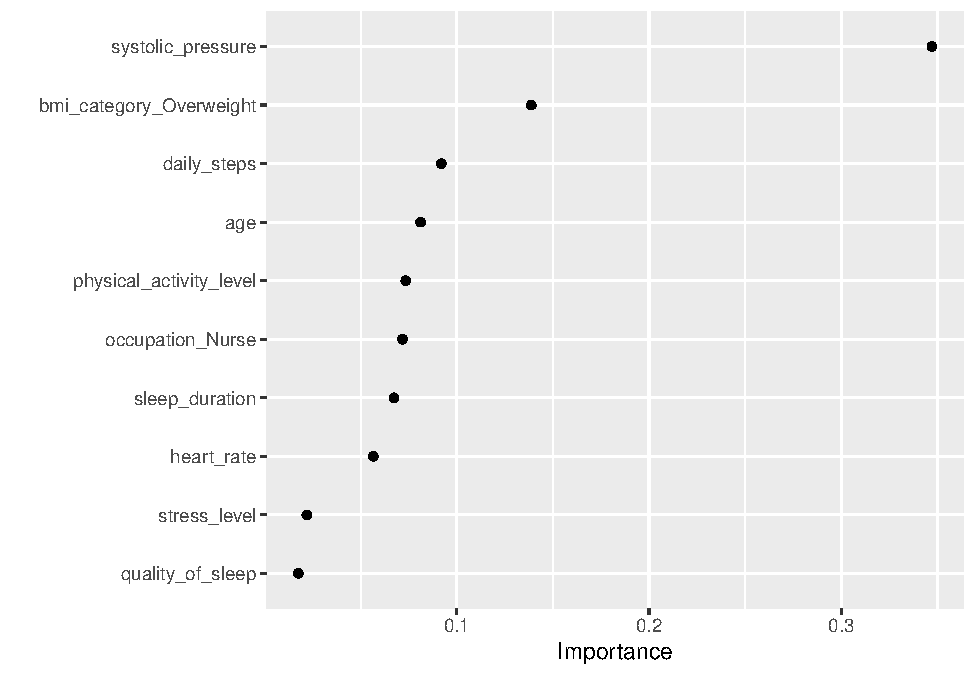
\includegraphics[width=0.6\linewidth]{projeto_files/figure-latex/pt. 4 -1} \end{center}

\end{document}
